\documentclass{article}
\usepackage{graphicx} % Required for inserting images
\usepackage{subfigure}
\usepackage{hyperref}
\title{Stock Price Prediction Using LSTM and Random
Forest Regressor with yFinance API data}
\author{ {\bfseries Team:}  Data Detectives \\ Milestone - 03 \\ \\ {\bfseries Team Members:} \\Greeshma Jale\\ Kalpana Bolla \\Meghala Anumolu\\Pravalika Bhupathi \\ Abhinaya Tanniru}



\begin{document}

\maketitle

\section{Introduction}
This technical document outlines the process of building a stock price prediction
model using Long Short-Term Memory (LSTM) neural networks and Random
Forest Regressor. The goal is to predict future stock prices based on historical
data and technical indicators.

\section{Data Collection and Preprocessing}

 {\bfseries Data Retrieval:} 
\begin{itemize}

  \item Historical stock data for Microsoft (MSFT) is obtained using the yfinance library and saved as a CSV file.

\end{itemize}
\begin{figure}
    \centering
    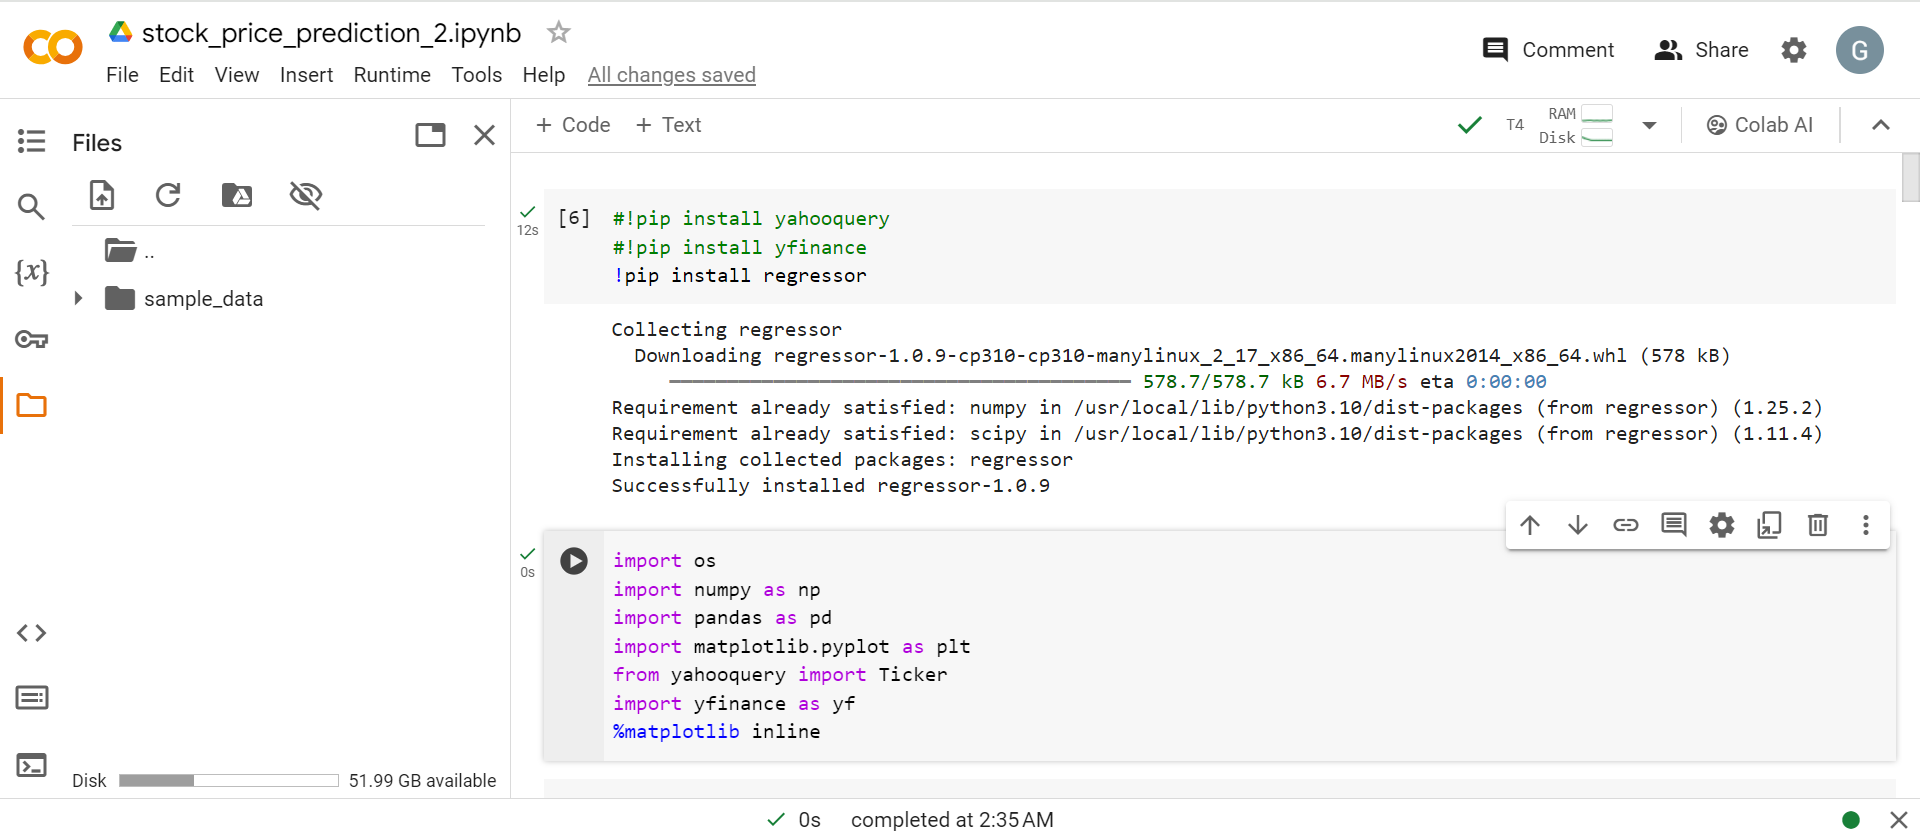
\includegraphics[width=1\linewidth]{Capture1.PNG}
    \caption{Data obtained from Yahoo Finance Library.}
    \label{fig:enter-label}
\end{figure}
     
\begin{figure}
    \centering
    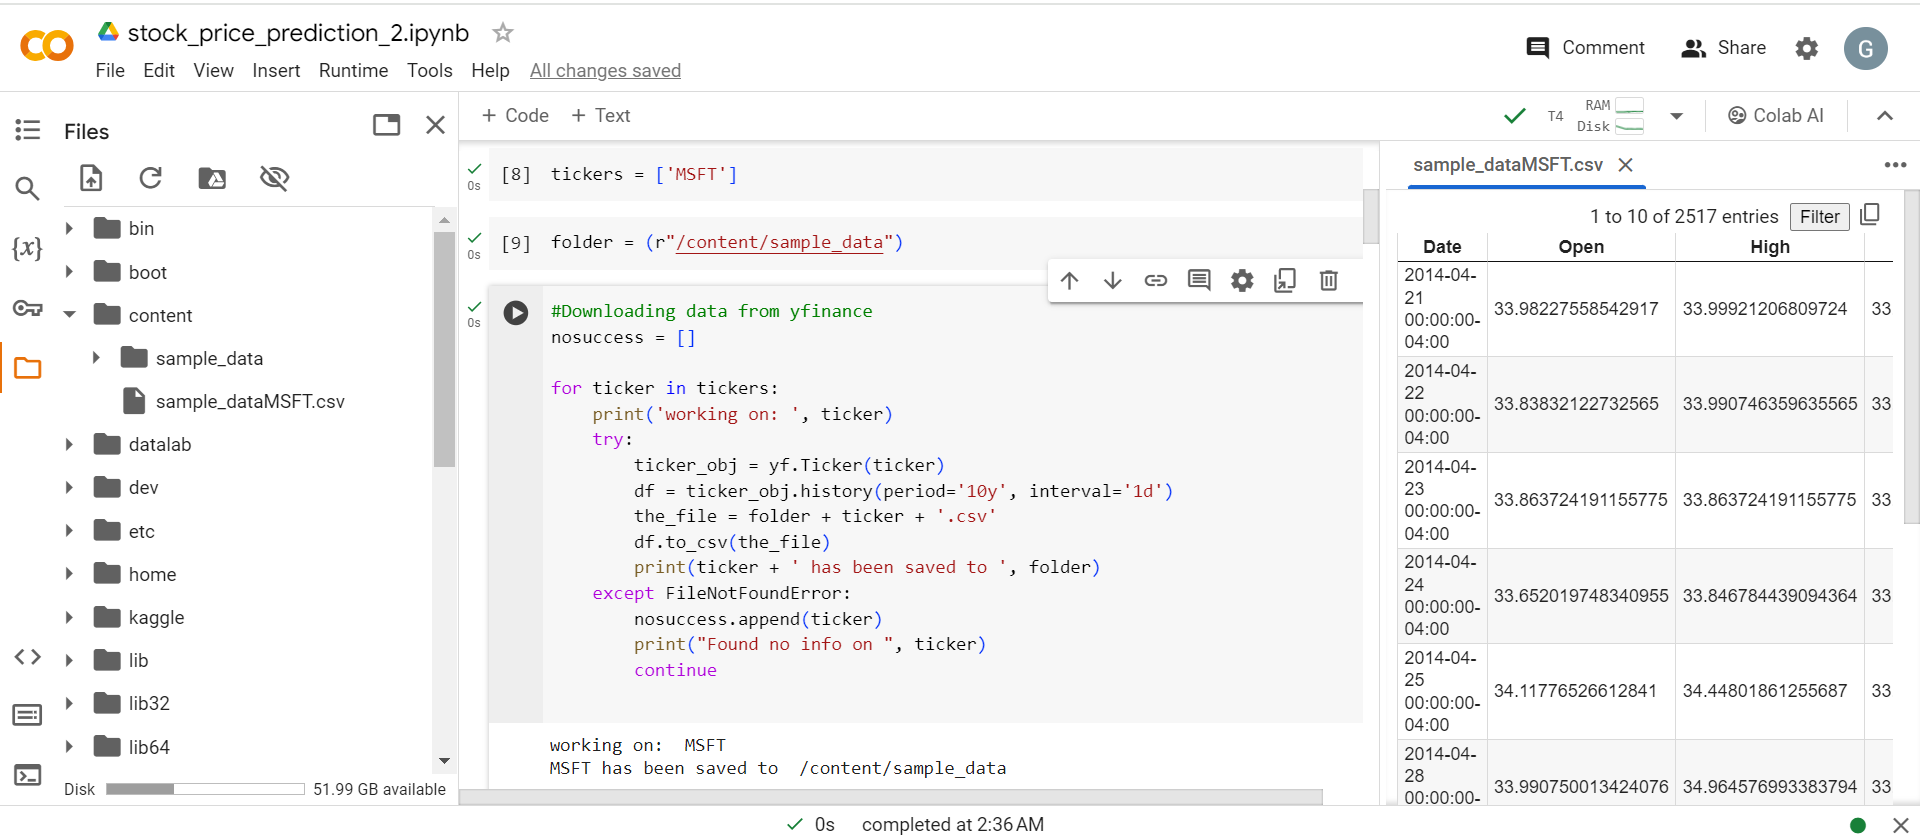
\includegraphics[width=1\linewidth]{Capture2.PNG}
    \caption{Fetched data saved as a CSV file.}
    \label{fig:enter-label}
\end{figure}

\noindent {\bfseries Data Splitting:}
\begin{itemize}
  \item The dataset is split into training (80\%) and test (20\%) sets and stored in separate CSV files.

\begin{figure}
    \centering
    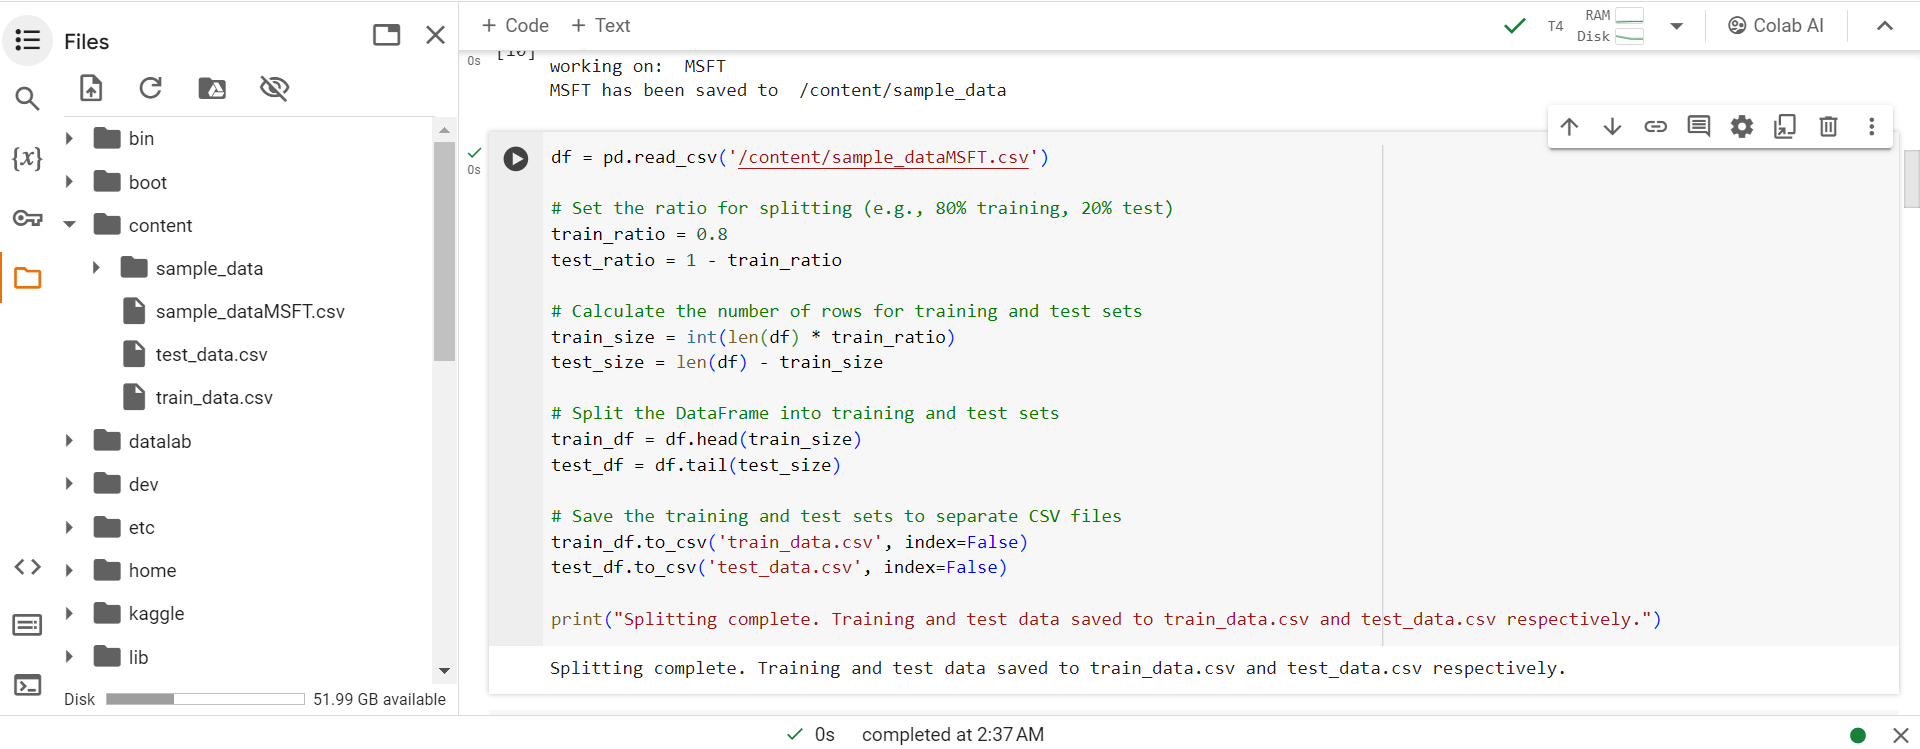
\includegraphics[width=1\linewidth]{Capture3.PNG}
    \caption{dataset is split into train and test sets and stored in
separate CSV files.}
    \label{fig:enter-label}
\end{figure}
\end{itemize}

 

\noindent {\bfseries Preprocessing: :} 
\begin{itemize}
 \item Numerical features are scaled using Min-Max scaling to a range of (0,1).
 \end{itemize}
 
 \begin{itemize}
 \item Technical indicators such as Moving Averages (MA) and Relative Strength
Index (RSI) are computed and added to the dataset.
  \end{itemize}

   \begin{itemize}
 \item Rows with missing values resulting from rolling calculations are dropped.
  \end{itemize}
  
 

  \begin{figure}
    \centering
    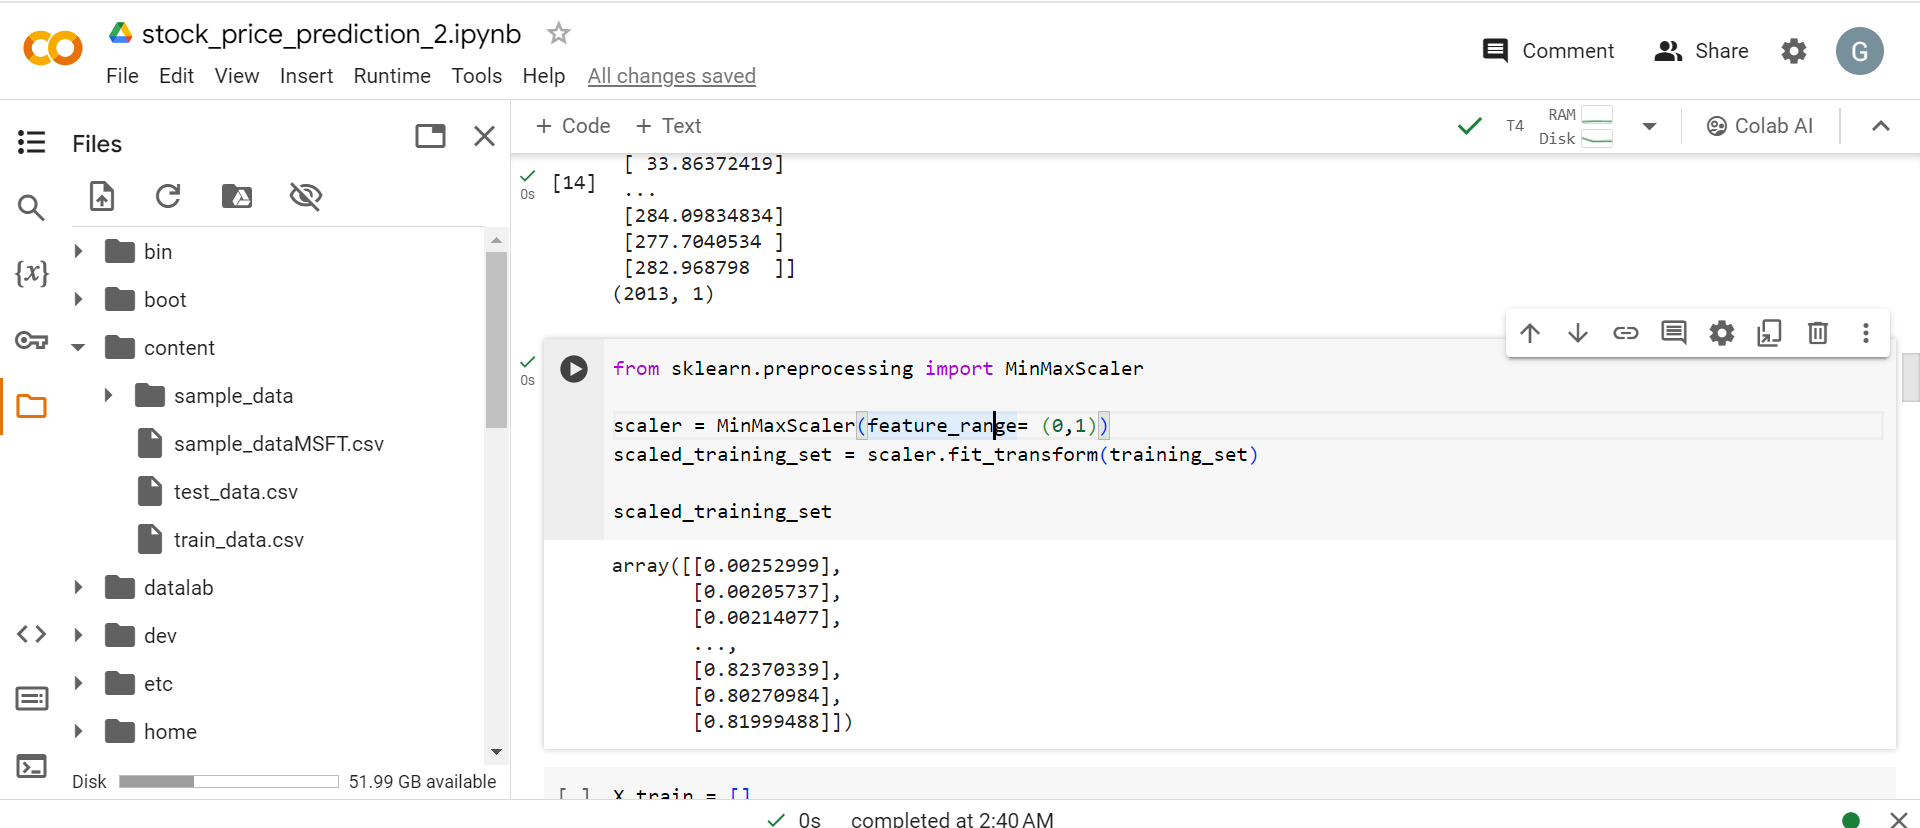
\includegraphics[width=1\linewidth]{Capture6.PNG}
    \caption{Numerical features are scaled using Min-Max scaling to a range of (0,1).}
    \label{fig:enter-label}
\end{figure}






\section{Model Preparation}
{\bfseries Long Short Term Memory (LSTM) 
} 

\noindent {\bfseries Architecture:}
\begin{itemize}
  \item Four LSTM layers with 50 units each are stacked, followed by a dropout rate of 0.2 after each LSTM layer to prevent overfitting.
  \begin{figure}
      \centering
      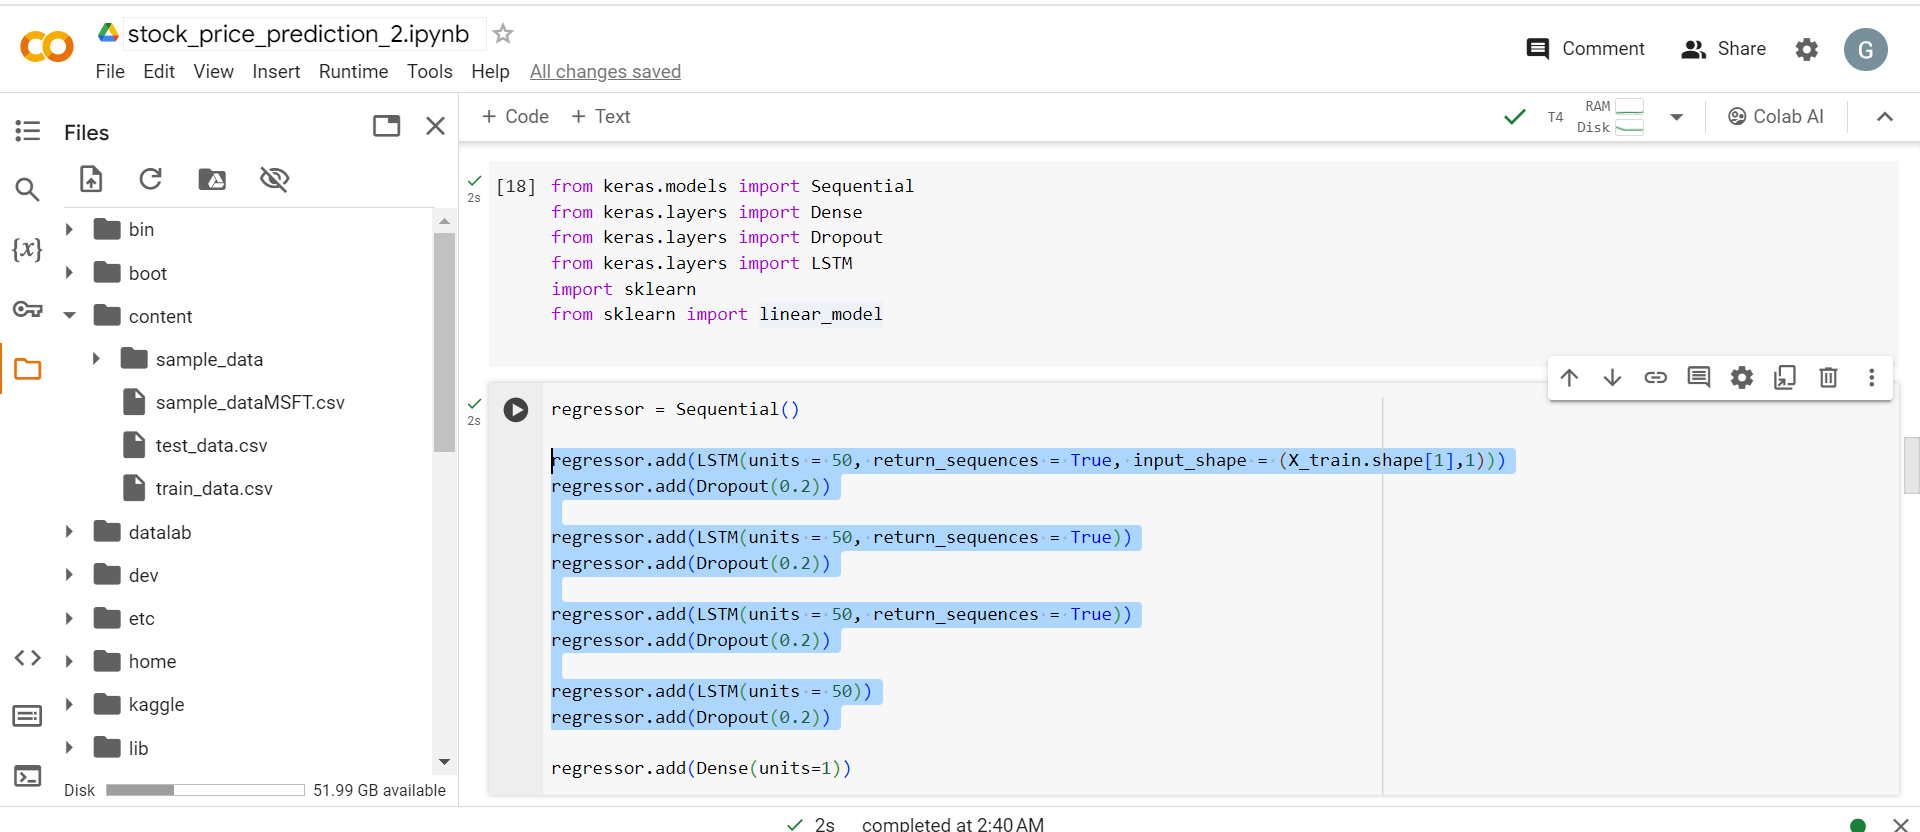
\includegraphics[width=1\linewidth]{Capture7.PNG}
      \caption{Four LSTM layers with 50 units each.}
      \label{fig:enter-label}
  \end{figure}
\item Input shape is defined based on the time steps and features of the training data (X\_train.shape[1], 1).
\end{itemize}

\noindent {\bfseries Compilation:}
\begin{itemize}
  \item The LSTM model is compiled using the Adam optimizer and Mean Squared Error
(MSE) loss function for regression tasks.
\begin{figure}
    \centering
    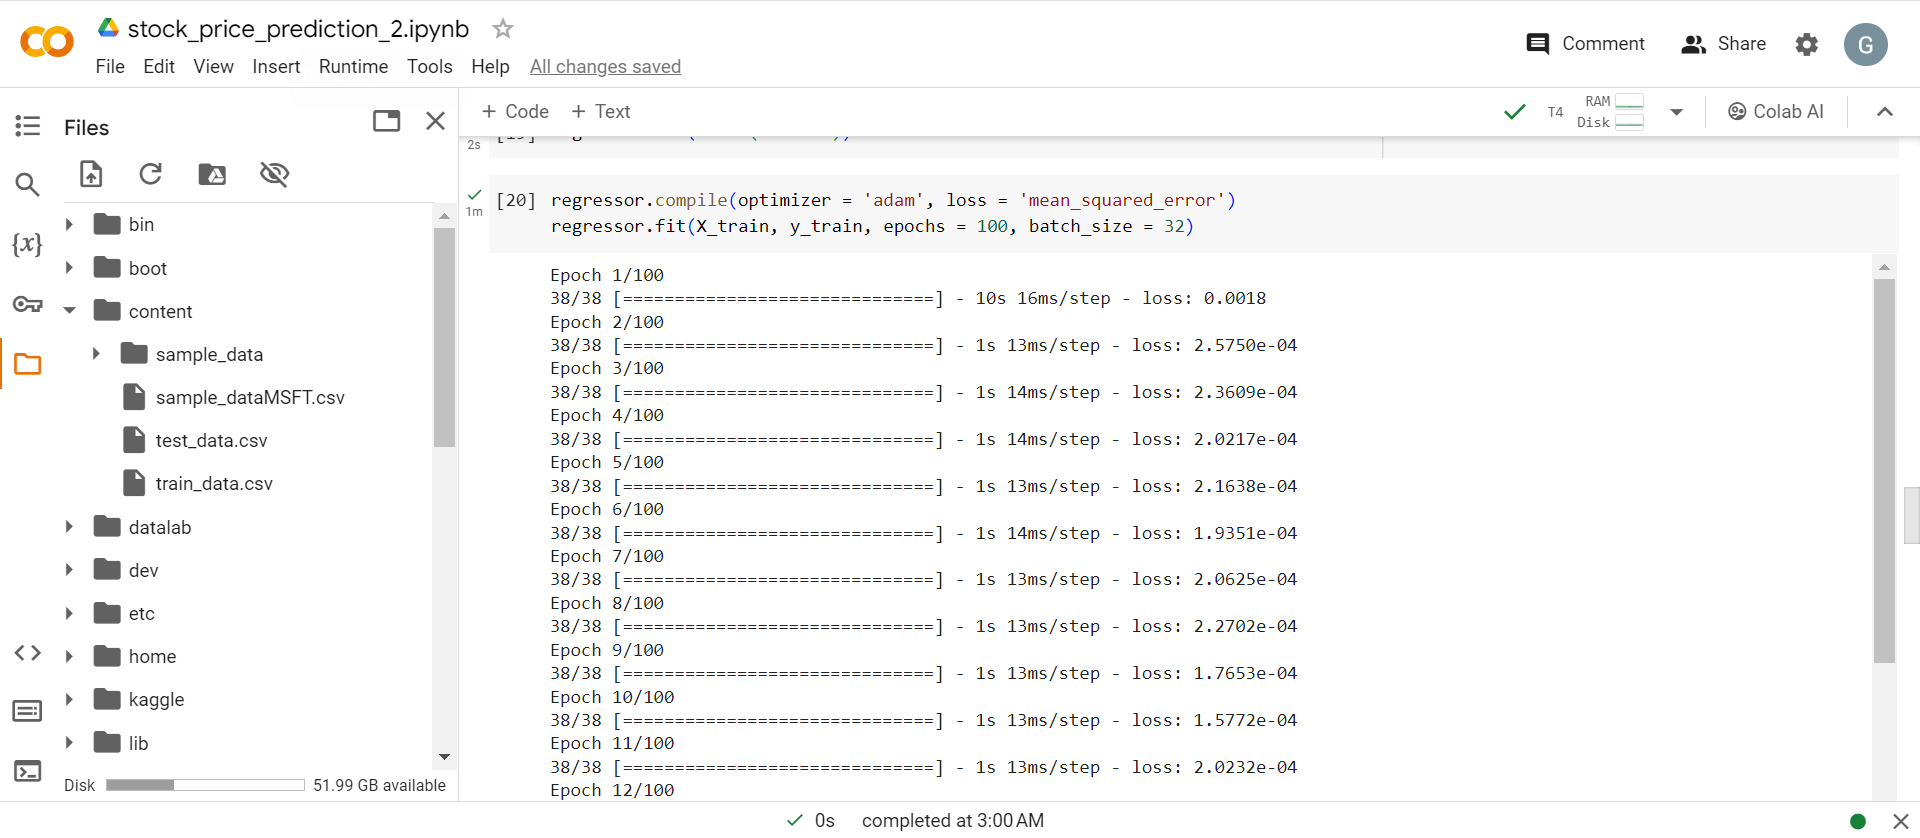
\includegraphics[width=1\linewidth]{Capture8.PNG}
    \caption{LSTM model is compiled using the Adam optimizer and Mean Squared
Error (MSE) loss function.}
    \label{fig:enter-label}
\end{figure}
\end{itemize}


\section{Training the LSTM Model}
{\bfseries Data Transformation: }
\begin{itemize}
  \item Training data is reshaped to fit the LSTM input shape (samples, time steps, features).

\end{itemize}

\noindent{\bfseries Training Process: }
\begin{itemize}
  \item The LSTM model is trained using the training data over 100 epochs with a batch size of 32 to learn temporal dependencies and predict future stock prices.

  \begin{figure}
      \centering
      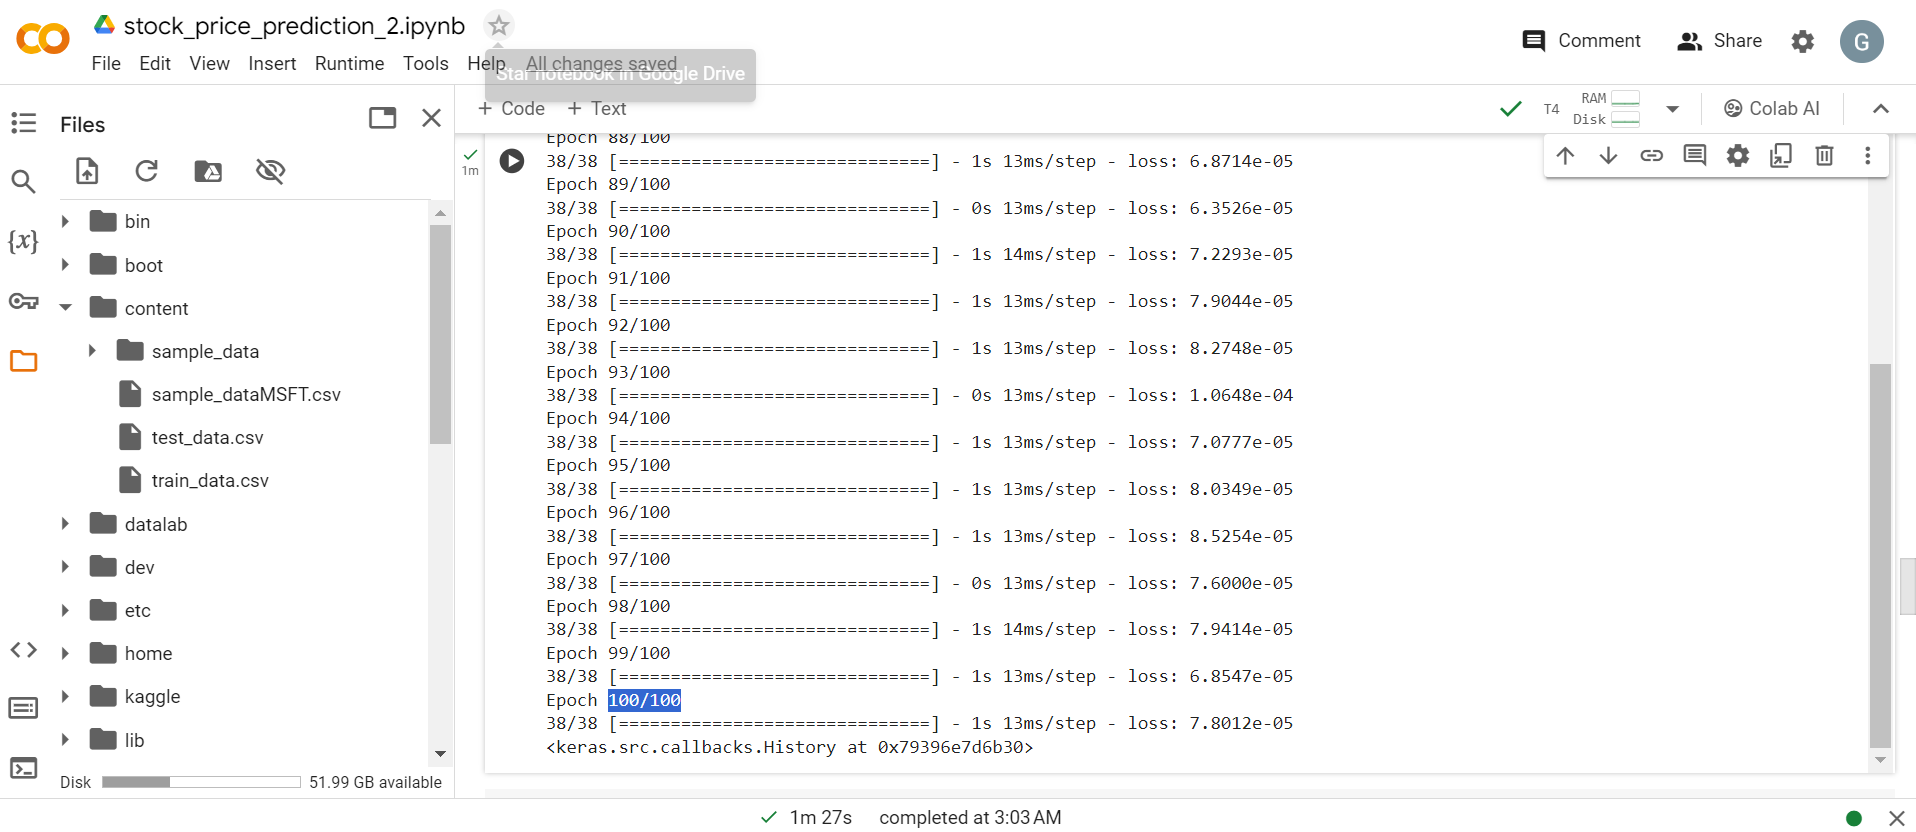
\includegraphics[width=1\linewidth]{Capture9.PNG}
      \caption{The LSTM model is trained using the training data over 100 epochs with a batch size of 32.}
      \label{fig:enter-label}
  \end{figure}
\end{itemize}
 
\section{Feature Engineering}
\noindent{\bfseries Additional Features: }
\begin{itemize}
  \item Technical features like Moving Averages (MA) and Relative Strength Index (RSI) are computed and included in the dataset.

\end{itemize}

\noindent{\bfseries Normalization: }
\begin{itemize}
  \item Numerical features are normalized using Min-Max scaling to ensure uniform feature ranges across the dataset.

\end{itemize}
 \begin{figure}
     \centering
     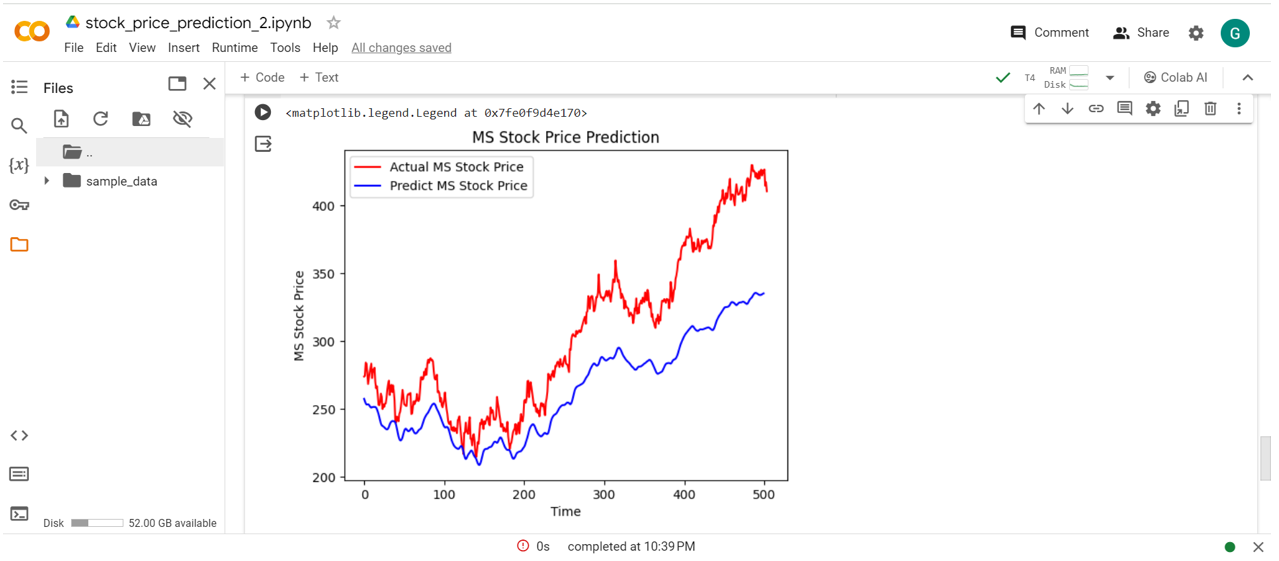
\includegraphics[width=1\linewidth]{Capture10.PNG}
     \caption{Graph showing the actual and predicted stock prices}
     \label{fig:enter-label}
 \end{figure}

\begin{figure}
    \centering
    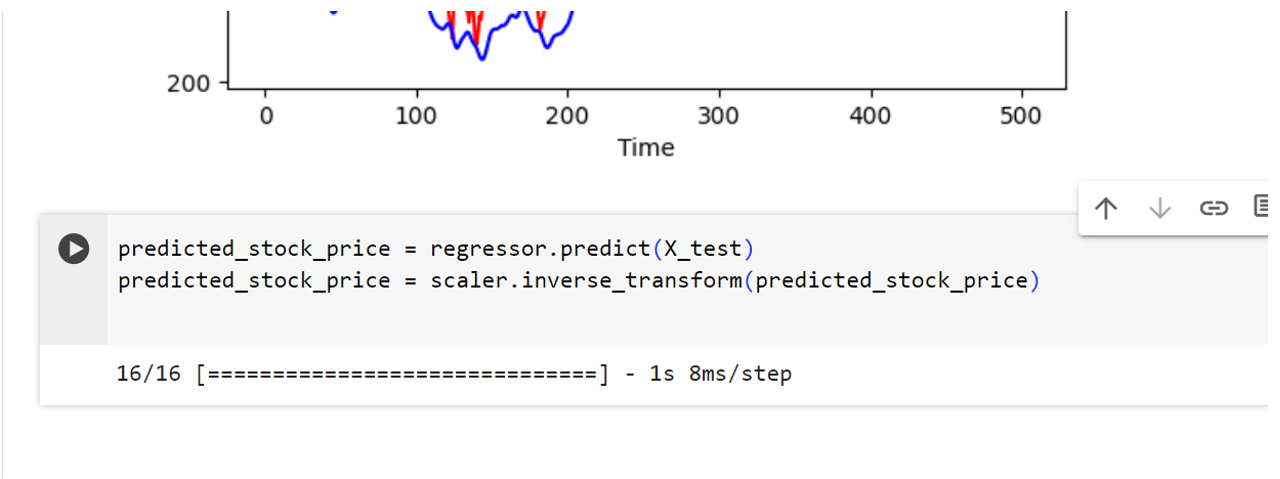
\includegraphics[width=1\linewidth]{Capture11.PNG}
    \caption{shows the number of batches processed (16/16) and the time taken per batch is indicated in milliseconds (8ms/step). }
    \label{fig:enter-label}
\end{figure}
\section{Training Random Forest Regressor}
\noindent{\bfseries Model Selection: }
\begin{itemize}
  \item  A Random Forest Regressor model from sklearn is trained using preprocessed features and target variables (closing prices).

\end{itemize}

\begin{figure}
    \centering
    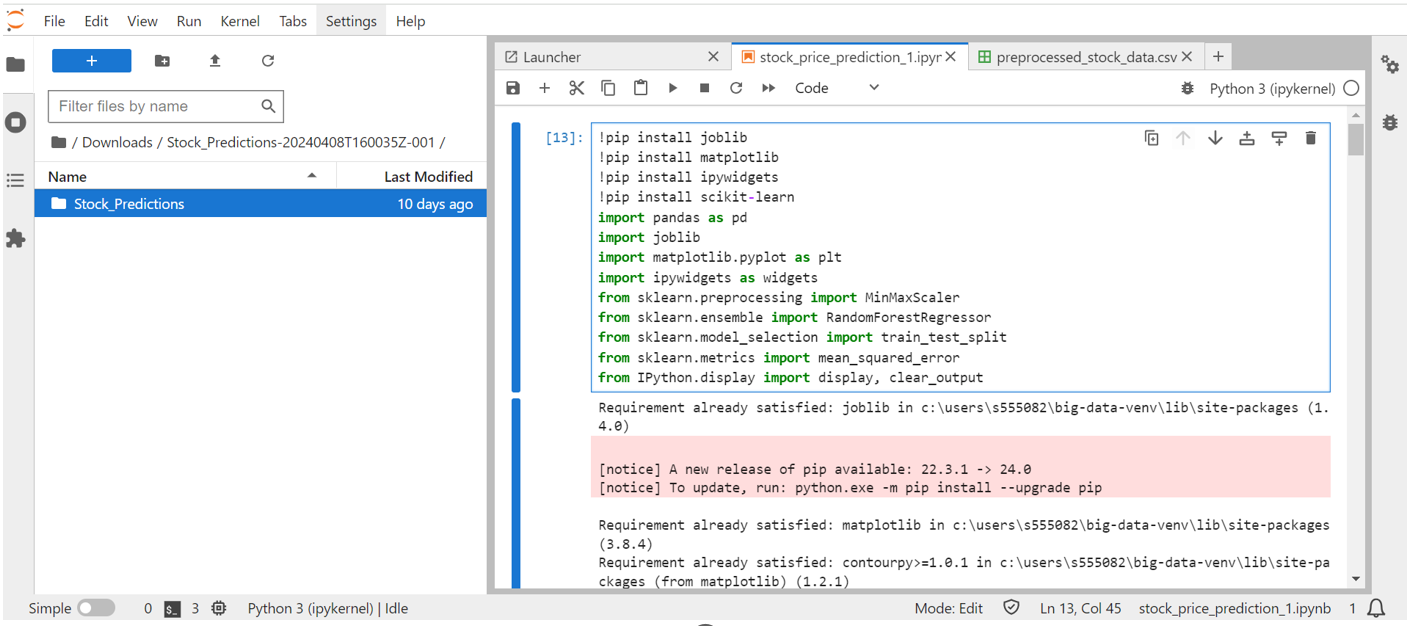
\includegraphics[width=1\linewidth]{Capture12.PNG}
    \caption{Packages for Random Forest Regressor sucessfully installed.}
    \label{fig:enter-label}
\end{figure}
\begin{figure}
    \centering
    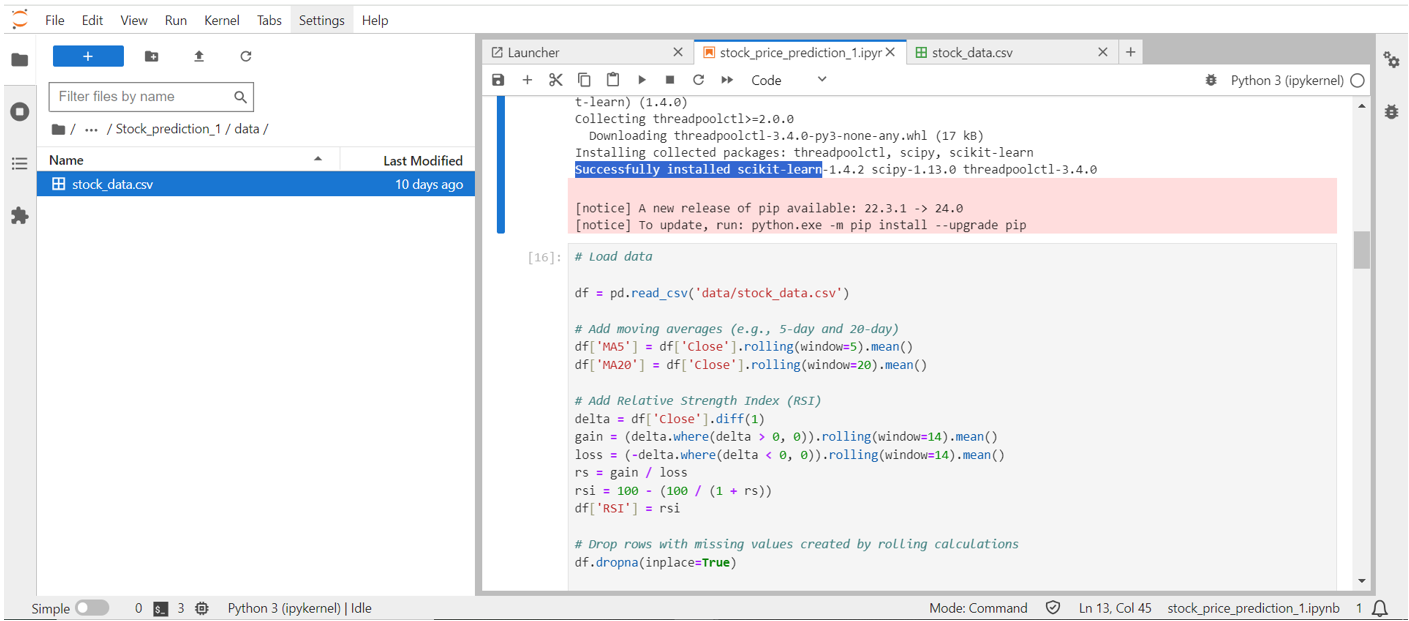
\includegraphics[width=1\linewidth]{Capture13.PNG}
    \caption{Loading MSFT stock data}
    \label{fig:enter-label}
\end{figure}
\begin{figure}
    \centering
    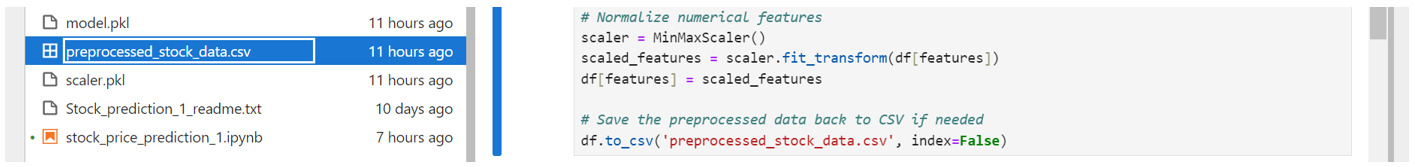
\includegraphics[width=1\linewidth]{Capture14.PNG}
    \caption{Preprocessed data generated.}
    \label{fig:enter-label}
\end{figure}
\noindent{\bfseries Model Configuration: }
\begin{itemize}
  \item   The Random Forest model is configured with 100 decision trees (n\_estimators=100) and a specified random state for reproducibility.

\end{itemize}


\section{Model Evaluation and Prediction}
\begin{figure}
    \centering
    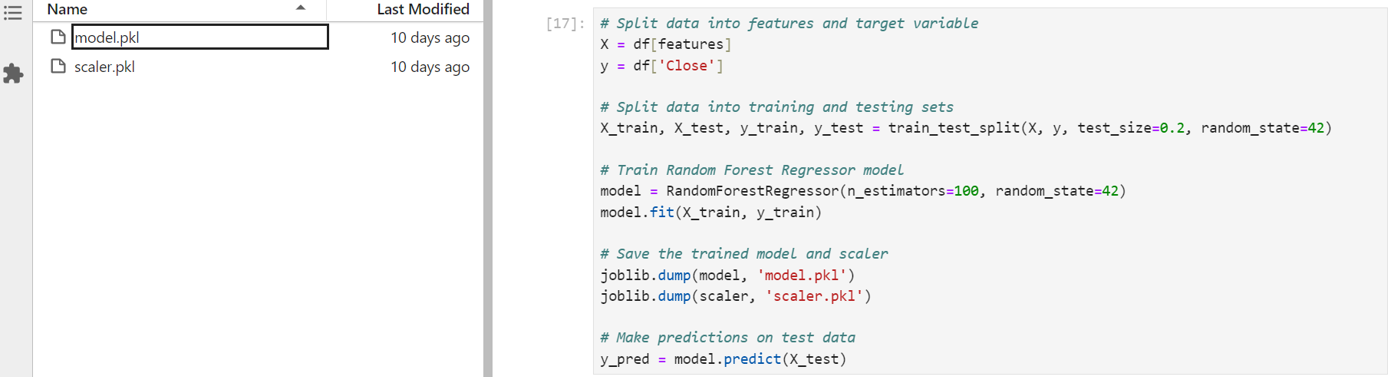
\includegraphics[width=1\linewidth]{Capture15.PNG}
    \caption{Splitting the dataset(train and test sets) and training the Random Forest Regressor Model.}
    \label{fig:enter-label}
\end{figure}
\begin{itemize}
    \item {\bfseries Model Saving:} Trained LSTM and Random Forest models, along with the scaler used for normalization, are saved for future use.
    \item {\bfseries Prediction Phase:} Predictions are generated on the test data using the trained Random Forest model to forecast future stock prices.
    \item {\bfseries Visualization:} Actual vs. predicted stock prices are plotted to evaluate model performance and accuracy in capturing stock price trends.
\end{itemize}

\begin{figure}
    \centering
    
    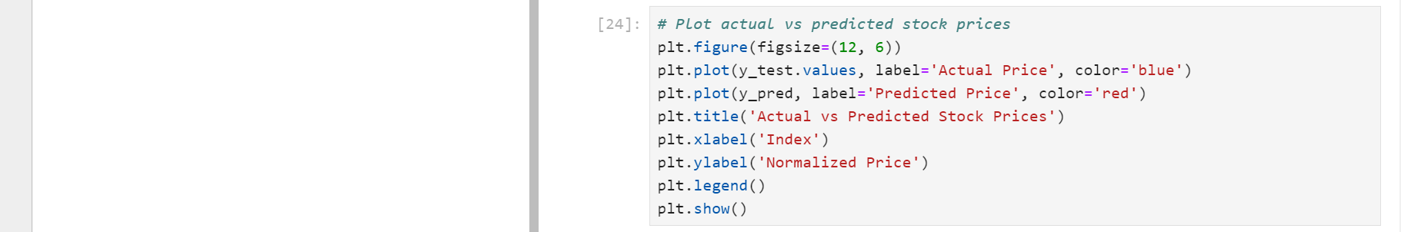
\includegraphics[width=1\linewidth]{Capture16.PNG}
    \begin{subfigure}
        \centering
        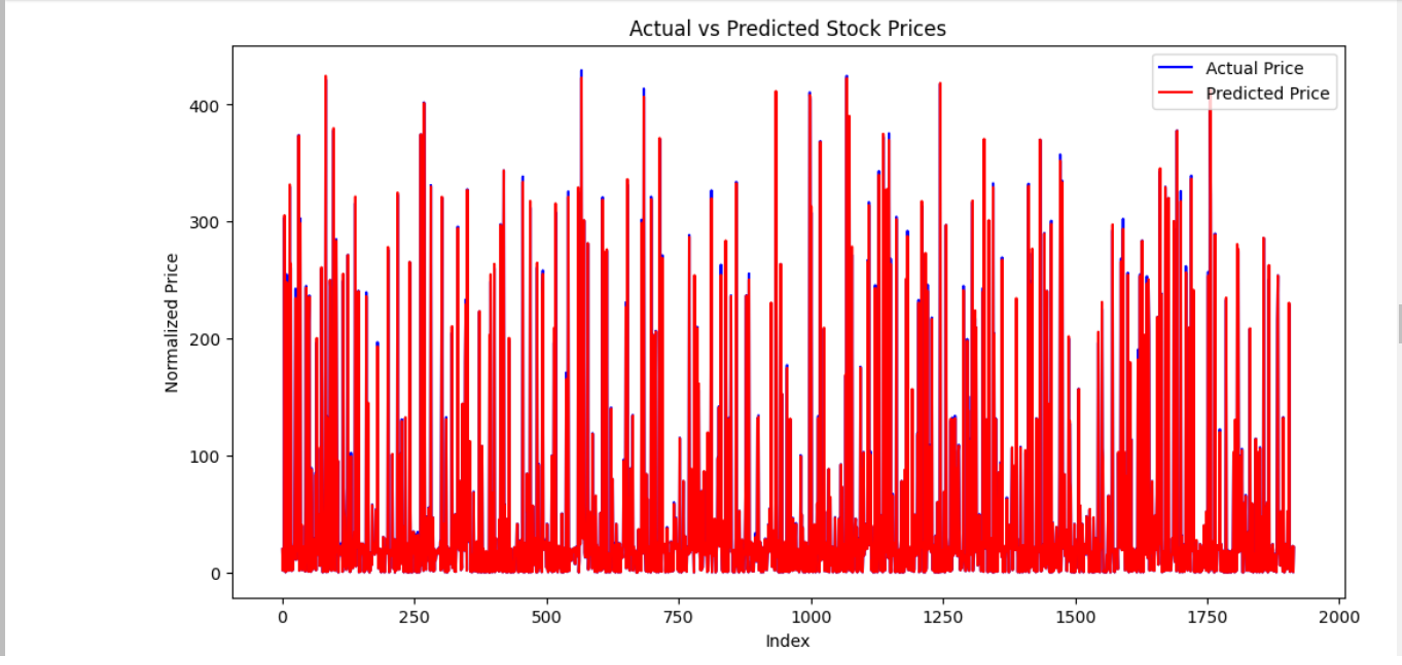
\includegraphics[width=\linewidth]{Capture17.PNG}
        \caption{Plotting actual vs Predicted stock prices.}
        \label{fig:subfig_a}
    \end{subfigure}
   
\end{figure}
\section{Setting up Python, jupyter lab, Google Colab }
\begin{itemize}
    \item {\bfseries Python Installation: }Download the Python installer from the official website, run it, and verify the installation by checking the Python version in PowerShell.
    \item {\bfseries Virtual Environment Setup:} After Python installation, create a virtual environment using python -m venv big-data-venv.
    \item {\bfseries Windows Terminal Installation:}  Download Windows Terminal from GitHub releases and install it with default options.
    \item {\bfseries Windows Terminal Configuration:} Open Windows Terminal, add a new profile, and modify the command line argument to include NoExit-File\%userprofile\%\textbackslash big-data-venv \textbackslash Scripts \textbackslash activate.ps1.
    \item {\bfseries JupyterLab Installation:} In the newly configured profile in Windows Terminal, install JupyterLab using pip install jupyterlab. If there are installation issues, try pip install jupyterlab==3.5.3 to resolve them.
    \item {\bfseries Accessing JupyterLab:} Launch JupyterLab by running jupyter lab and access it via localhost:8888/lab in a web browser.
    \item {\bfseries Setting Google Colab:}
    To open and import a dataset in Google Colab, you can follow these steps. First, open Google Colab by navigating to https://colab.research.google.com/ in your web browser. Once the Colab interface loads, create a new notebook by clicking on the "File" menu and selecting "New notebook." Next, you can import datasets into your Colab notebook from various sources such as Google Drive, GitHub, or directly from your local machine. 

\end{itemize}
\section{Metrics}
\begin{itemize}
    \item  {\bfseries Data Quality: }  The project ensures data quality by retrieving accurate historical stock data from a reliable source (Yahoo Finance), splitting the dataset into complete training and test sets, and applying consistent preprocessing steps to handle missing values and scale numerical features.
    \item {\bfseries 5Vs (Volume, Velocity, Variety, Veracity, Value):}  Volume: historical stock data for Microsoft (MSFT) using the yfinance library. Veracity:  preprocessed data. Value: accurately forecasting future stock prices based on historical data and technical indicators.

    \item {\bfseries Processing Time:} Used machine learning models to handle and process large datasets effectively.
    \item {\bfseries Resource Utilization: } Resource utilization in this project is optimized to ensure efficient usage of memory and computational resources during model training and evaluation, maximizing performance while minimizing resource wastage.
    \item {\bfseries Security: }  Security measures such as data encryption, access control, and regular updates are implemented to ensure the confidentiality and integrity of sensitive data used in the stock price prediction framework.
    \item {\bfseries  Cost:} Involves the time and resources required for data collection, preprocessing, model training, and evaluation.
\end{itemize}


\section{Conclusion}
\begin{itemize}
    \item {\bfseries  Data Preprocessing:}  Data preprocessing is essential for ensuring data quality and preparing it for model training.
    \item {\bfseries  Model Construction:} Building models using LSTM and Random Forest allows for capturing temporal dependencies and non-linear relationships in the data.
    \item {\bfseries  Feature Engineering:} Feature engineering enriches the dataset with additional insights, aiding in capturing important patterns and trends.
    \item {\bfseries Training Methodologies:}  Training methodologies, including configuration of layers and optimization techniques, are crucial for effective model learning.
    \item {\bfseries Model Evaluation and Prediction: }  Model evaluation through metrics and visualization provides insights into the accuracy and effectiveness of the predictive framework.
    \item {\bfseries Robust Framework:}   Usage of LSTM and Random Forest models offers a robust and versatile framework for stock price prediction.
\end{itemize}
\section{Citations:}
\begin{itemize}
\item {\bfseries  Python Reference:}
\url{https://docs.python.org/3/reference/index.html}
\item {\bfseries  Git URL:}
\url{https://github.com/KalpanaBolla/StockPricePrediction}
\item {\bfseries  Google Colab:}
\url{https://colab.google/}
\end{itemize}
\end{document}
